\documentclass{article}
\usepackage{style-notes}


\title{MATH 320: Probability\\Completed Notes}
\author{Colton Gearhart}
\date{\today}							

\begin{document}
\setcounter{secnumdepth}{0}		% trick to get unnumbered sections in table of contents
\maketitle
\dosecttoc
\tableofcontents
\newpage

%-------------------------------------------------------------------------
\section{Test 1}
%-------------------------------------------------------------------------

\secttoc

%----------------------------
\subsection{Lecture 0 -- Course Overview}
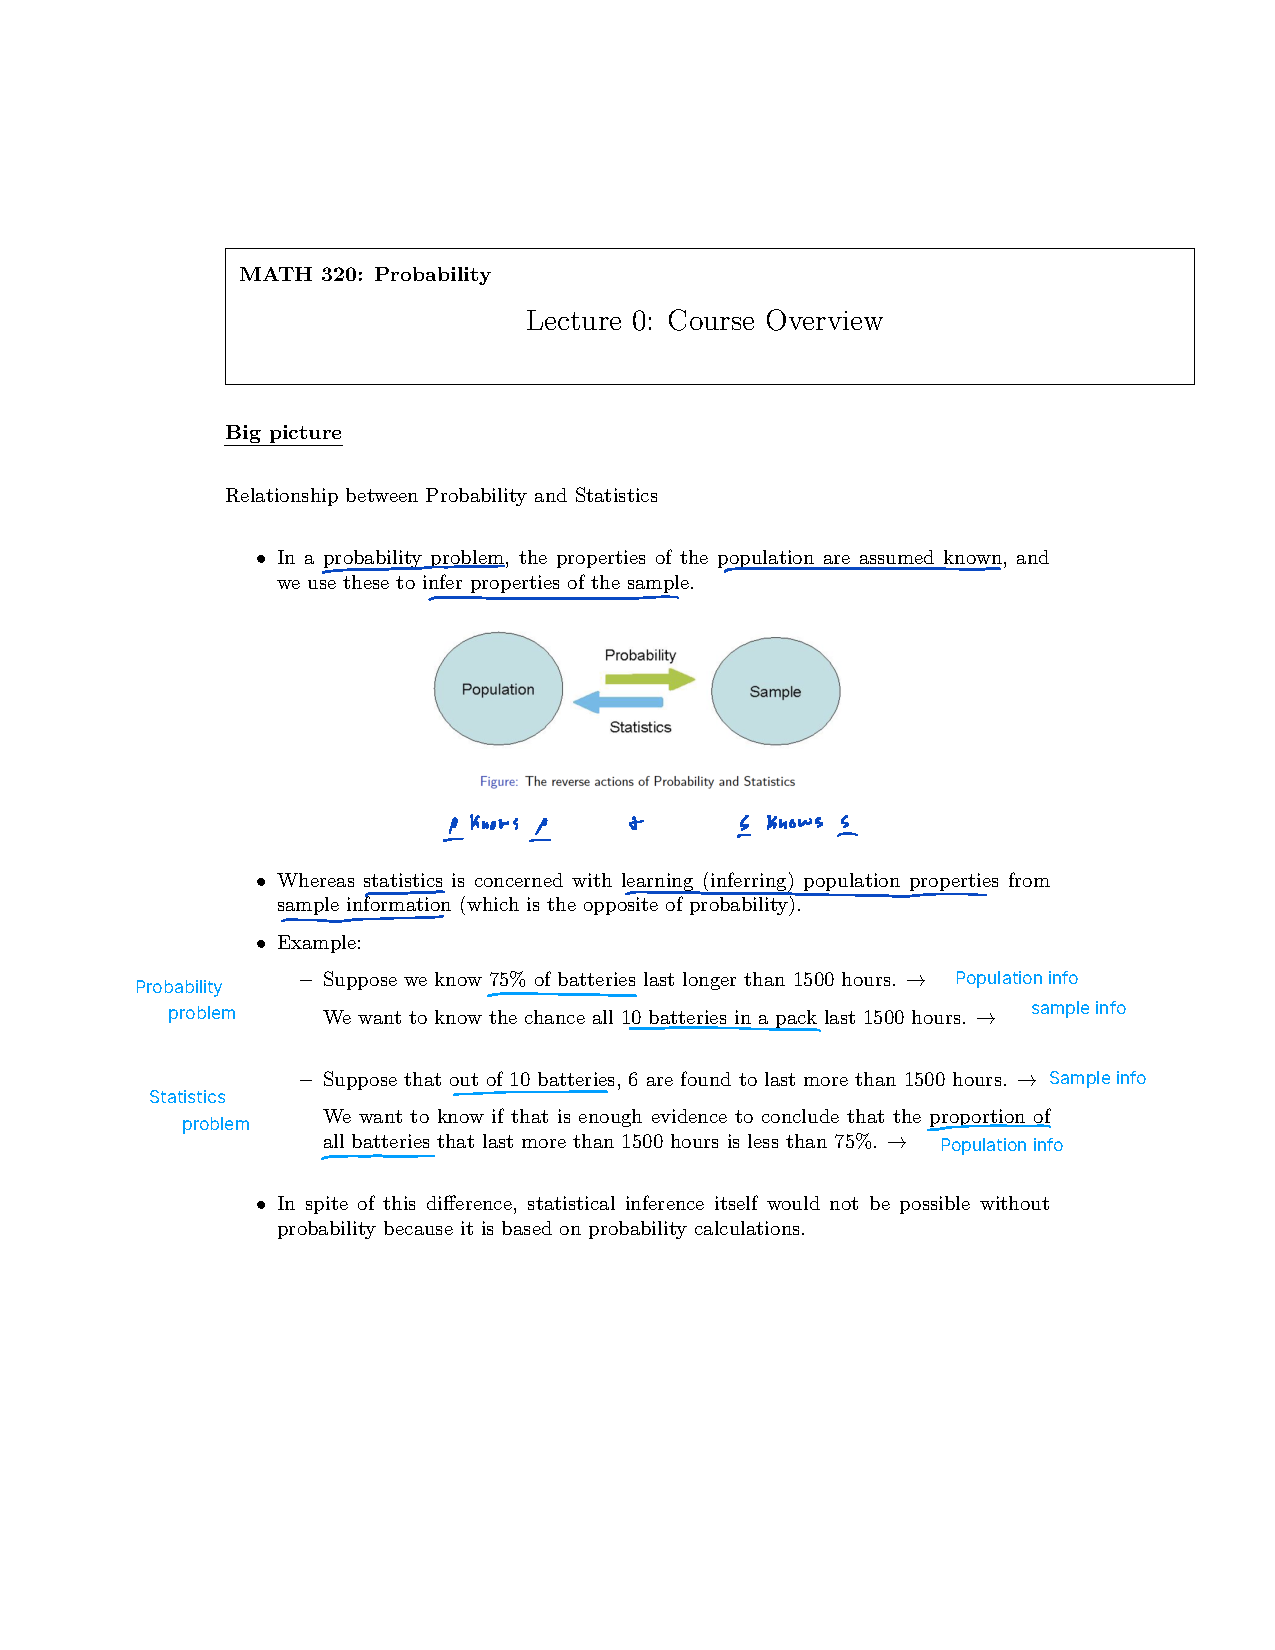
\includepdf[pages=-]{lecture-0-COMPLETED.pdf}\newpage
%----------------------------

%----------------------------
\subsection{Lecture 1 -- Set Theory}
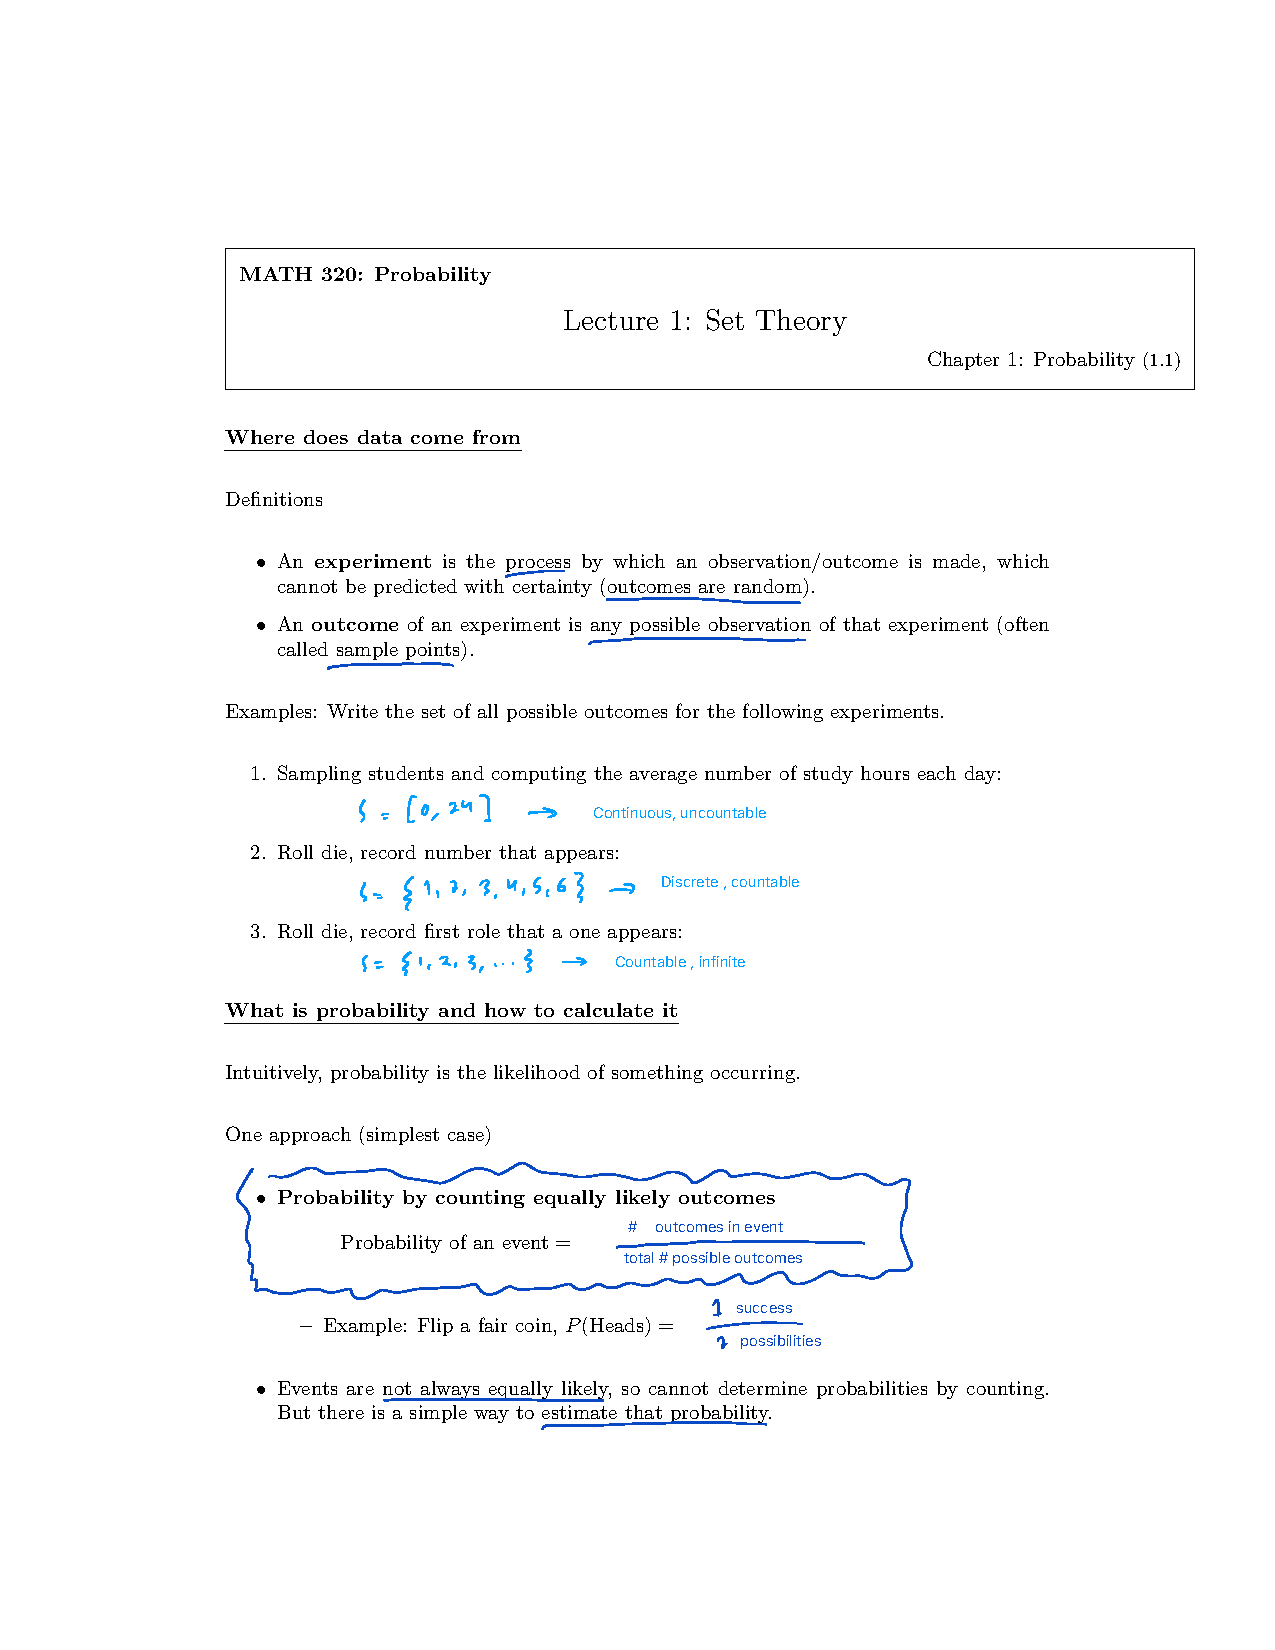
\includepdf[pages=-]{lecture-1-COMPLETED.pdf}\newpage
%----------------------------

%----------------------------
\subsection{Lecture 2 -- Counting}
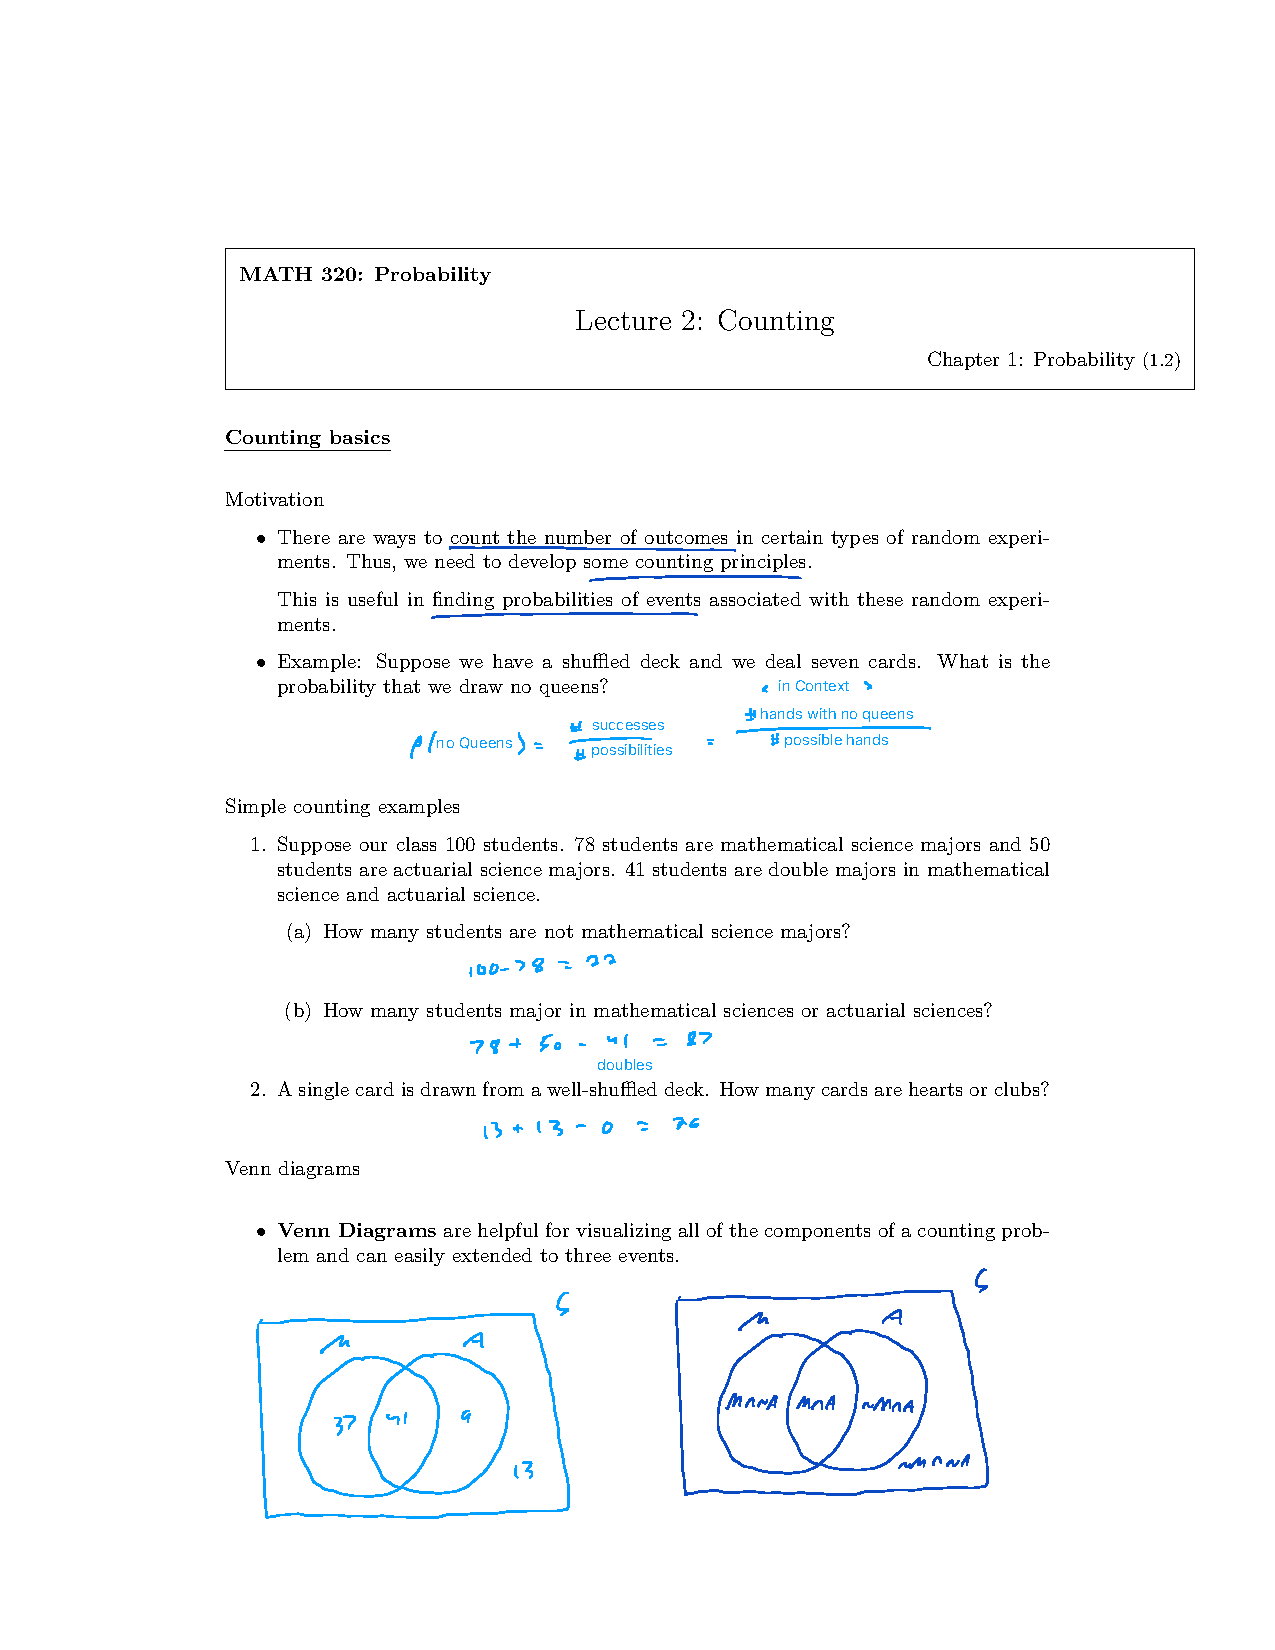
\includepdf[pages=-]{lecture-2-COMPLETED.pdf}\newpage
%----------------------------

%----------------------------
\subsection{Lecture 3 -- Probability}
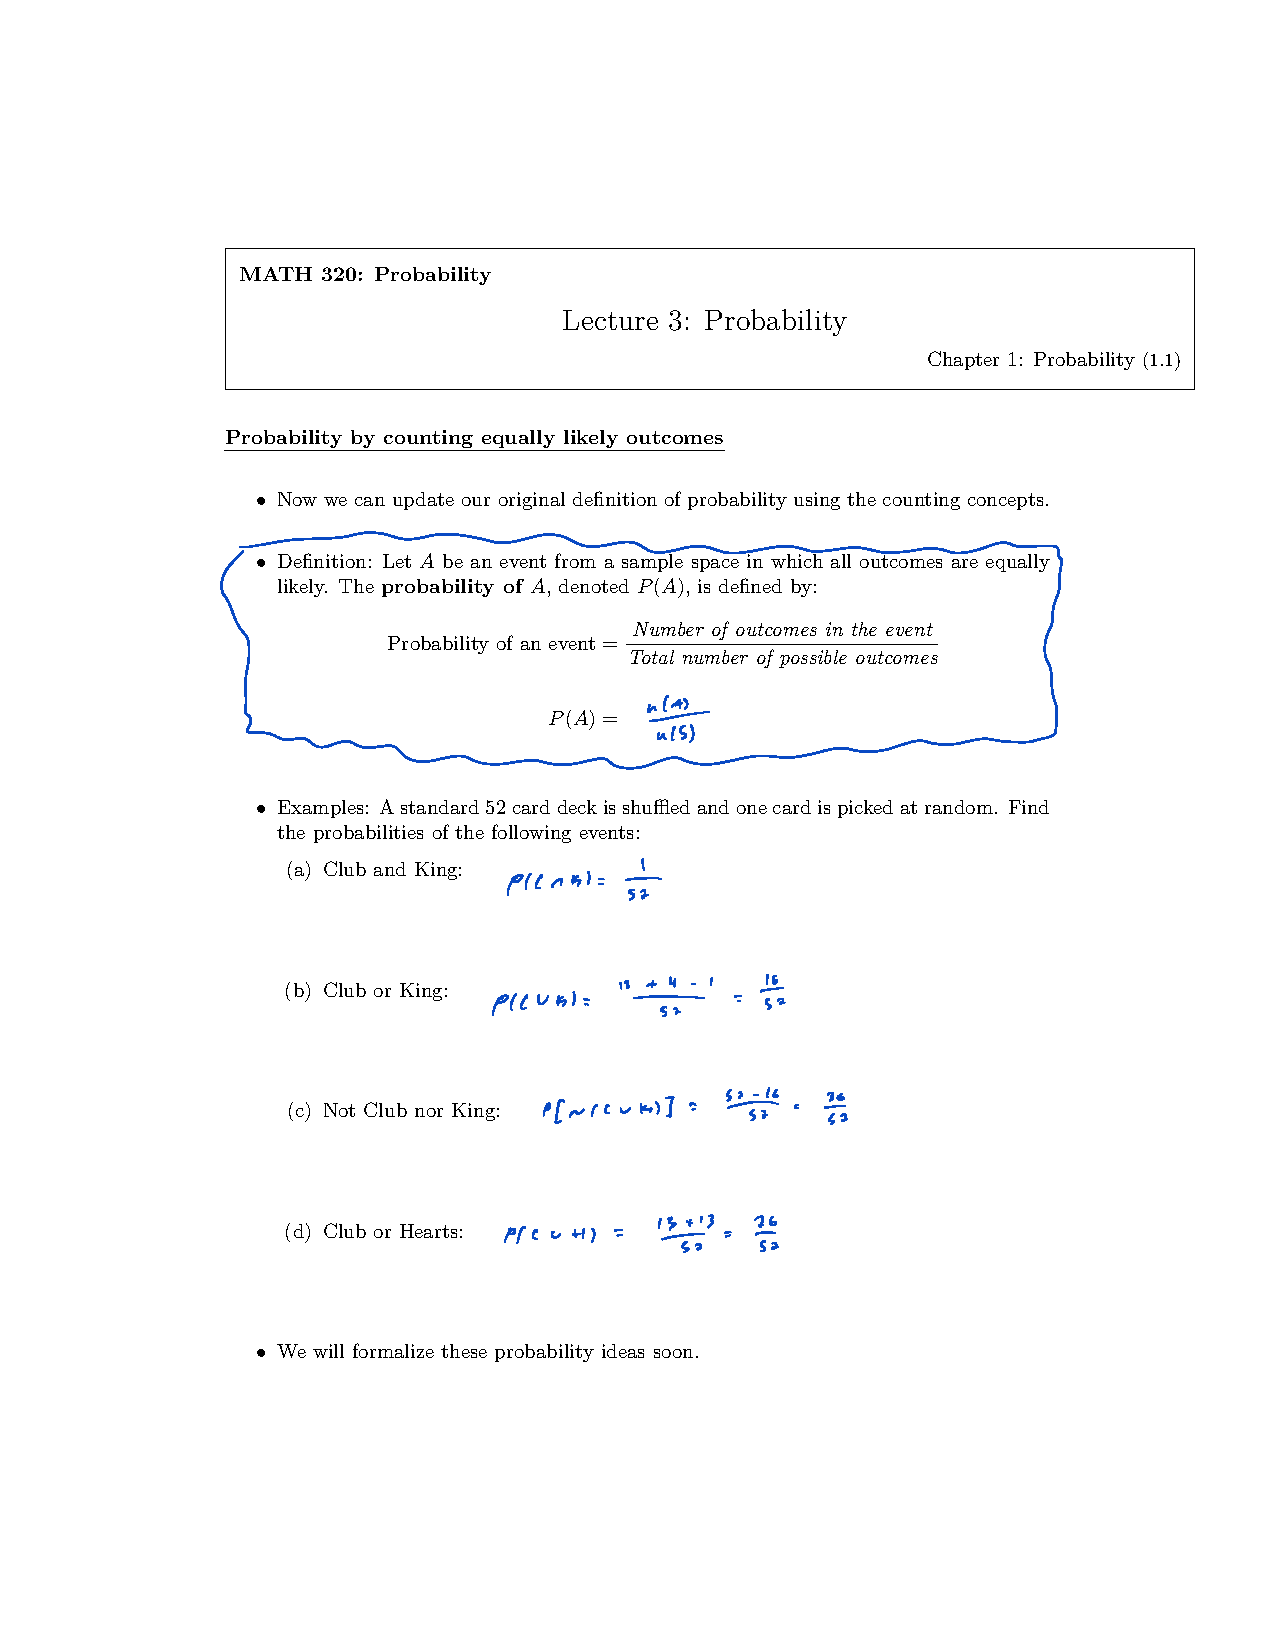
\includepdf[pages=-]{lecture-3-COMPLETED.pdf}\newpage
%----------------------------

%----------------------------
\subsection{Lecture 4 -- Conditional Probability}
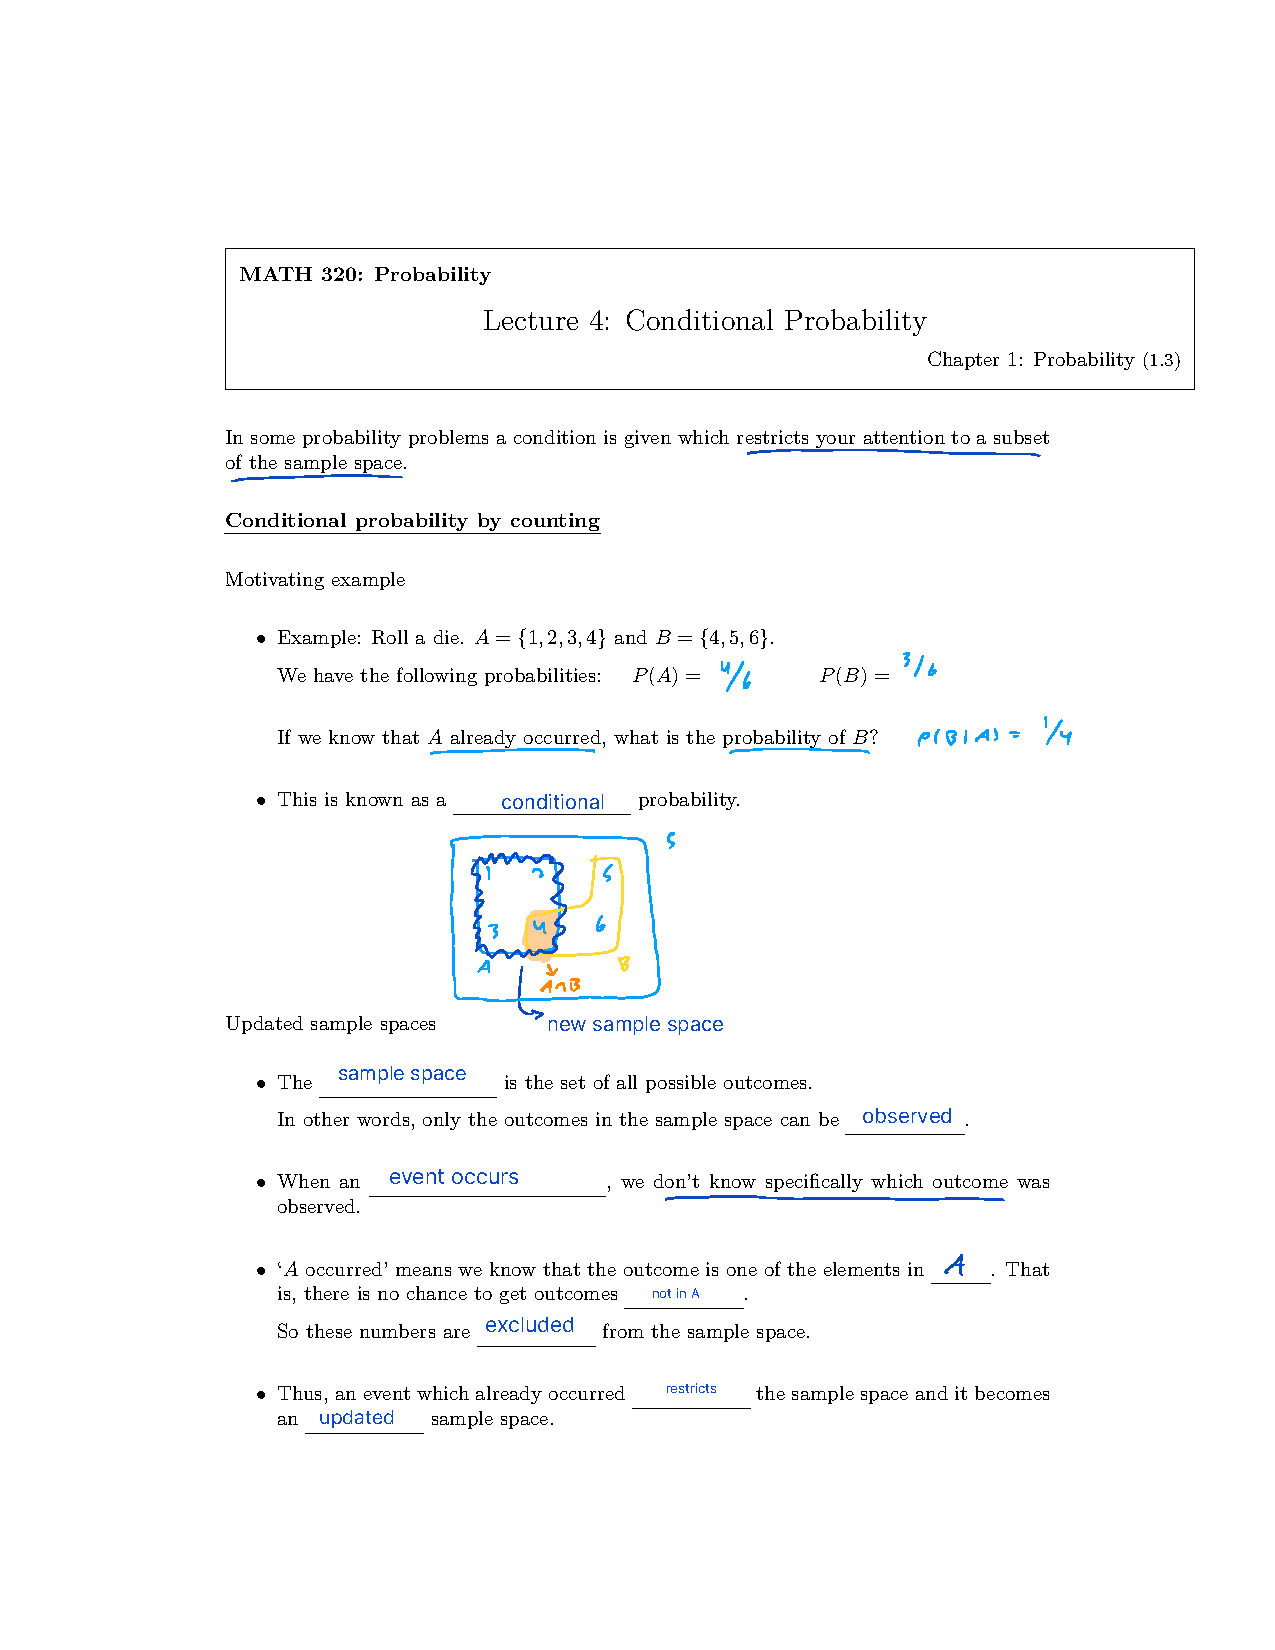
\includepdf[pages=-]{lecture-4-COMPLETED.pdf}\newpage
%----------------------------

%----------------------------
\subsection{Lecture 5 -- Independent Events}
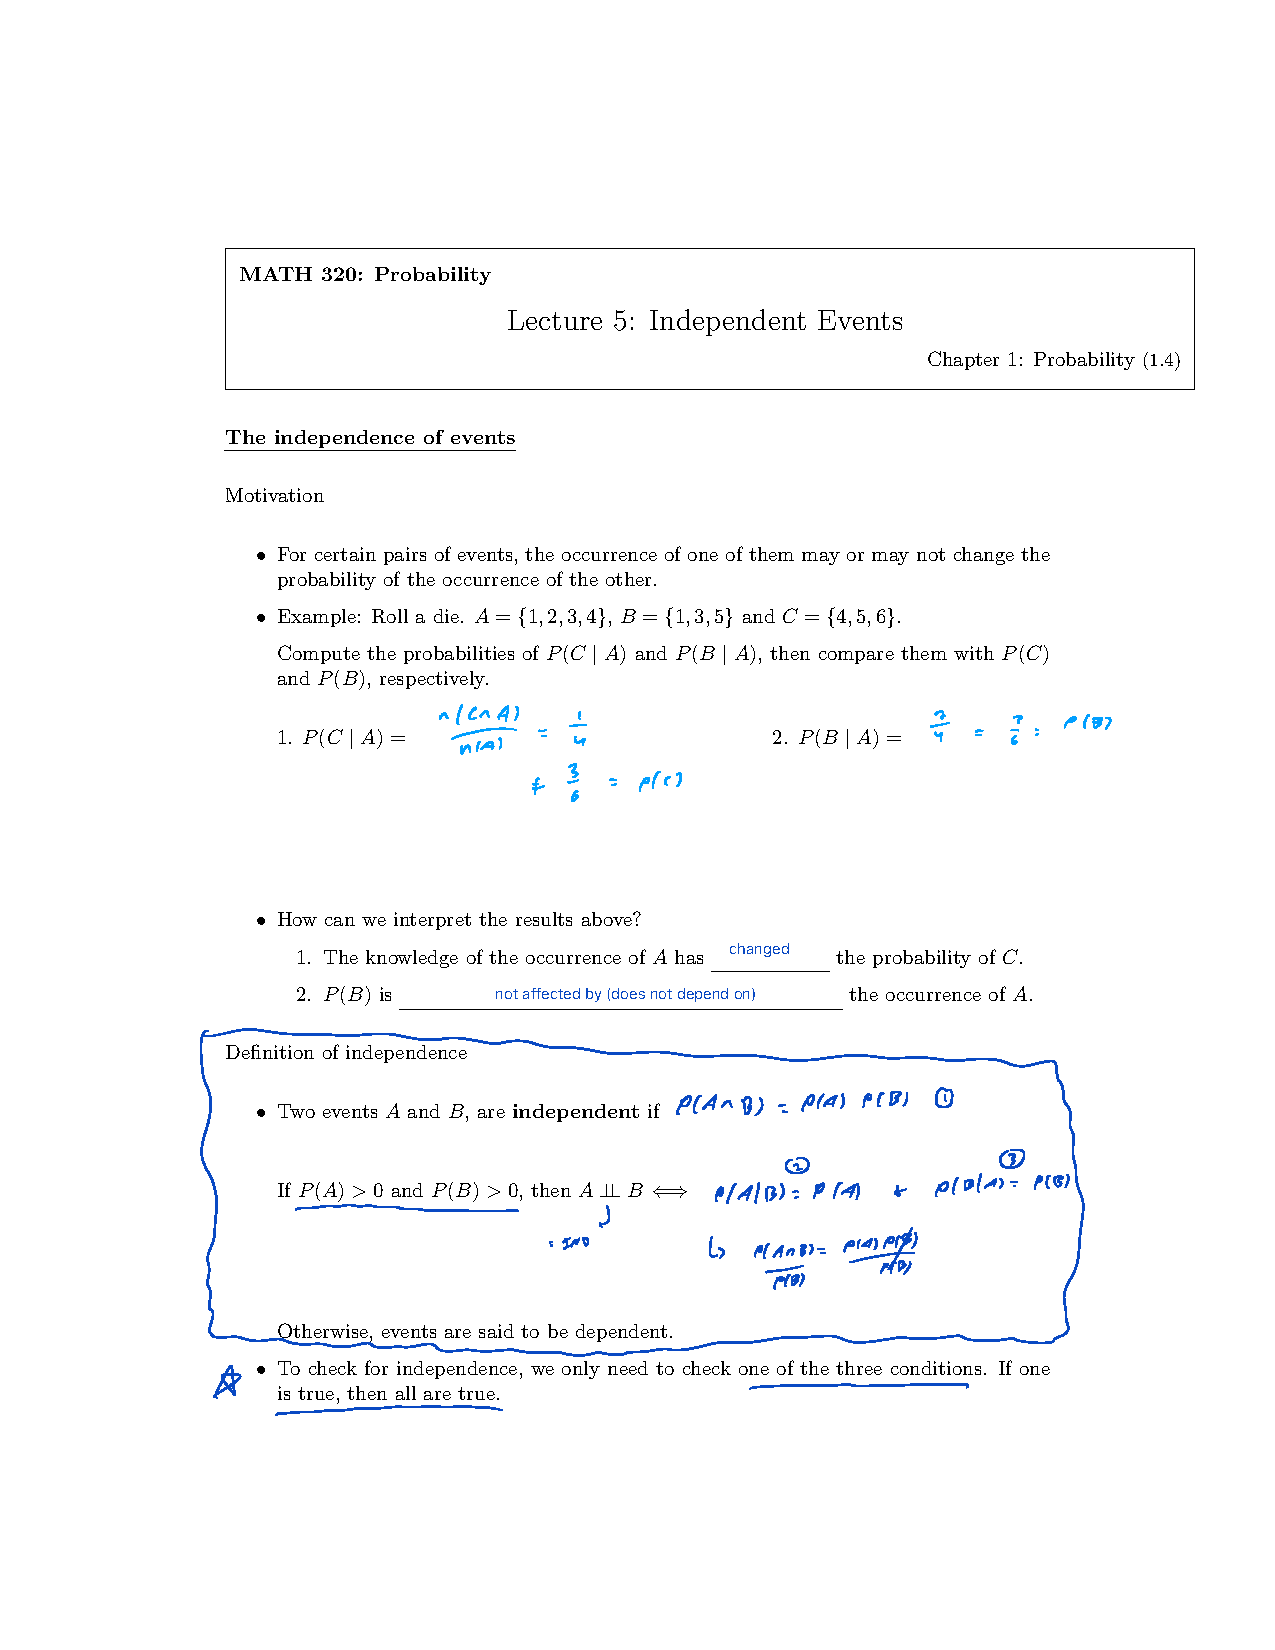
\includepdf[pages=-]{lecture-5-COMPLETED.pdf}\newpage
%----------------------------

%----------------------------
\subsection{Lecture 6 -- Bayes' Theorem}
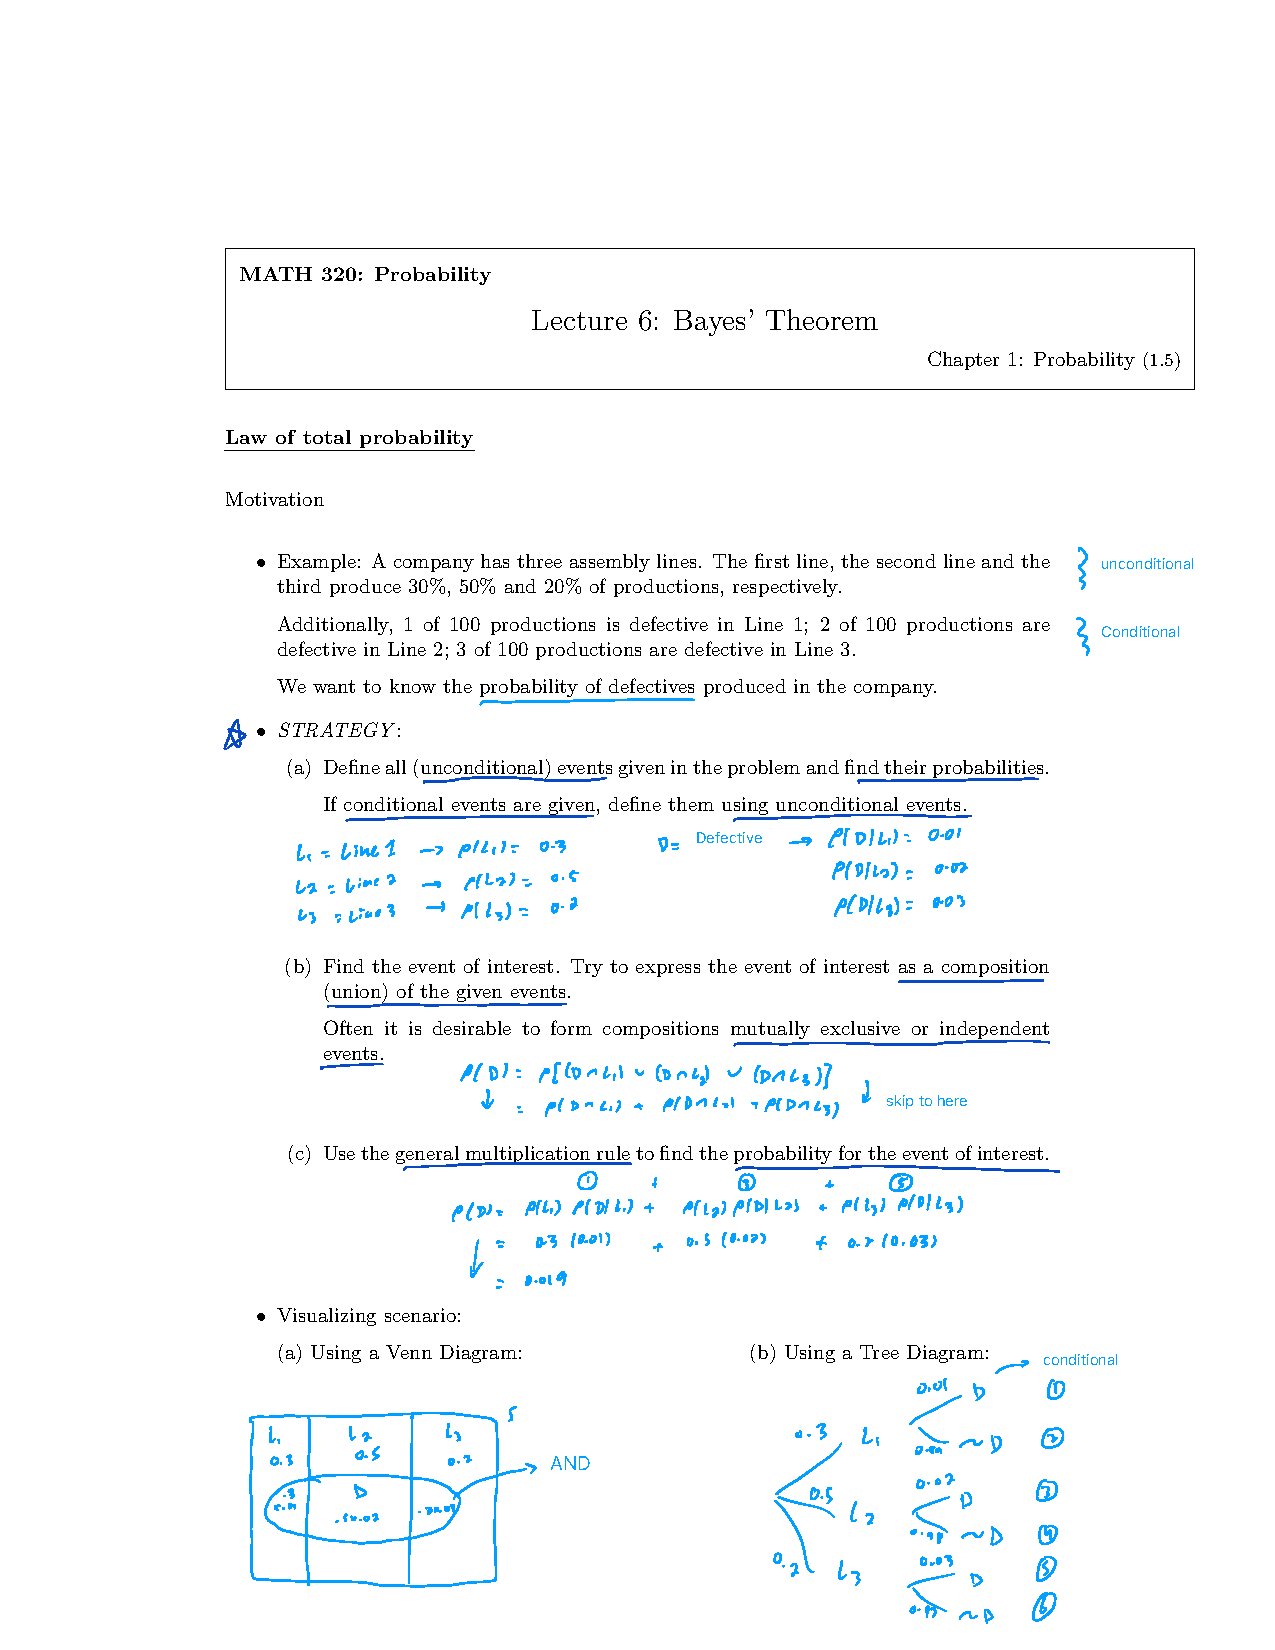
\includepdf[pages=-]{lecture-6-COMPLETED.pdf}\newpage
%----------------------------

%-------------------------------------------------------------------------
\section{Test 2}
%-------------------------------------------------------------------------

\secttoc

%----------------------------
\subsection{Lecture 7 -- Random Variables}
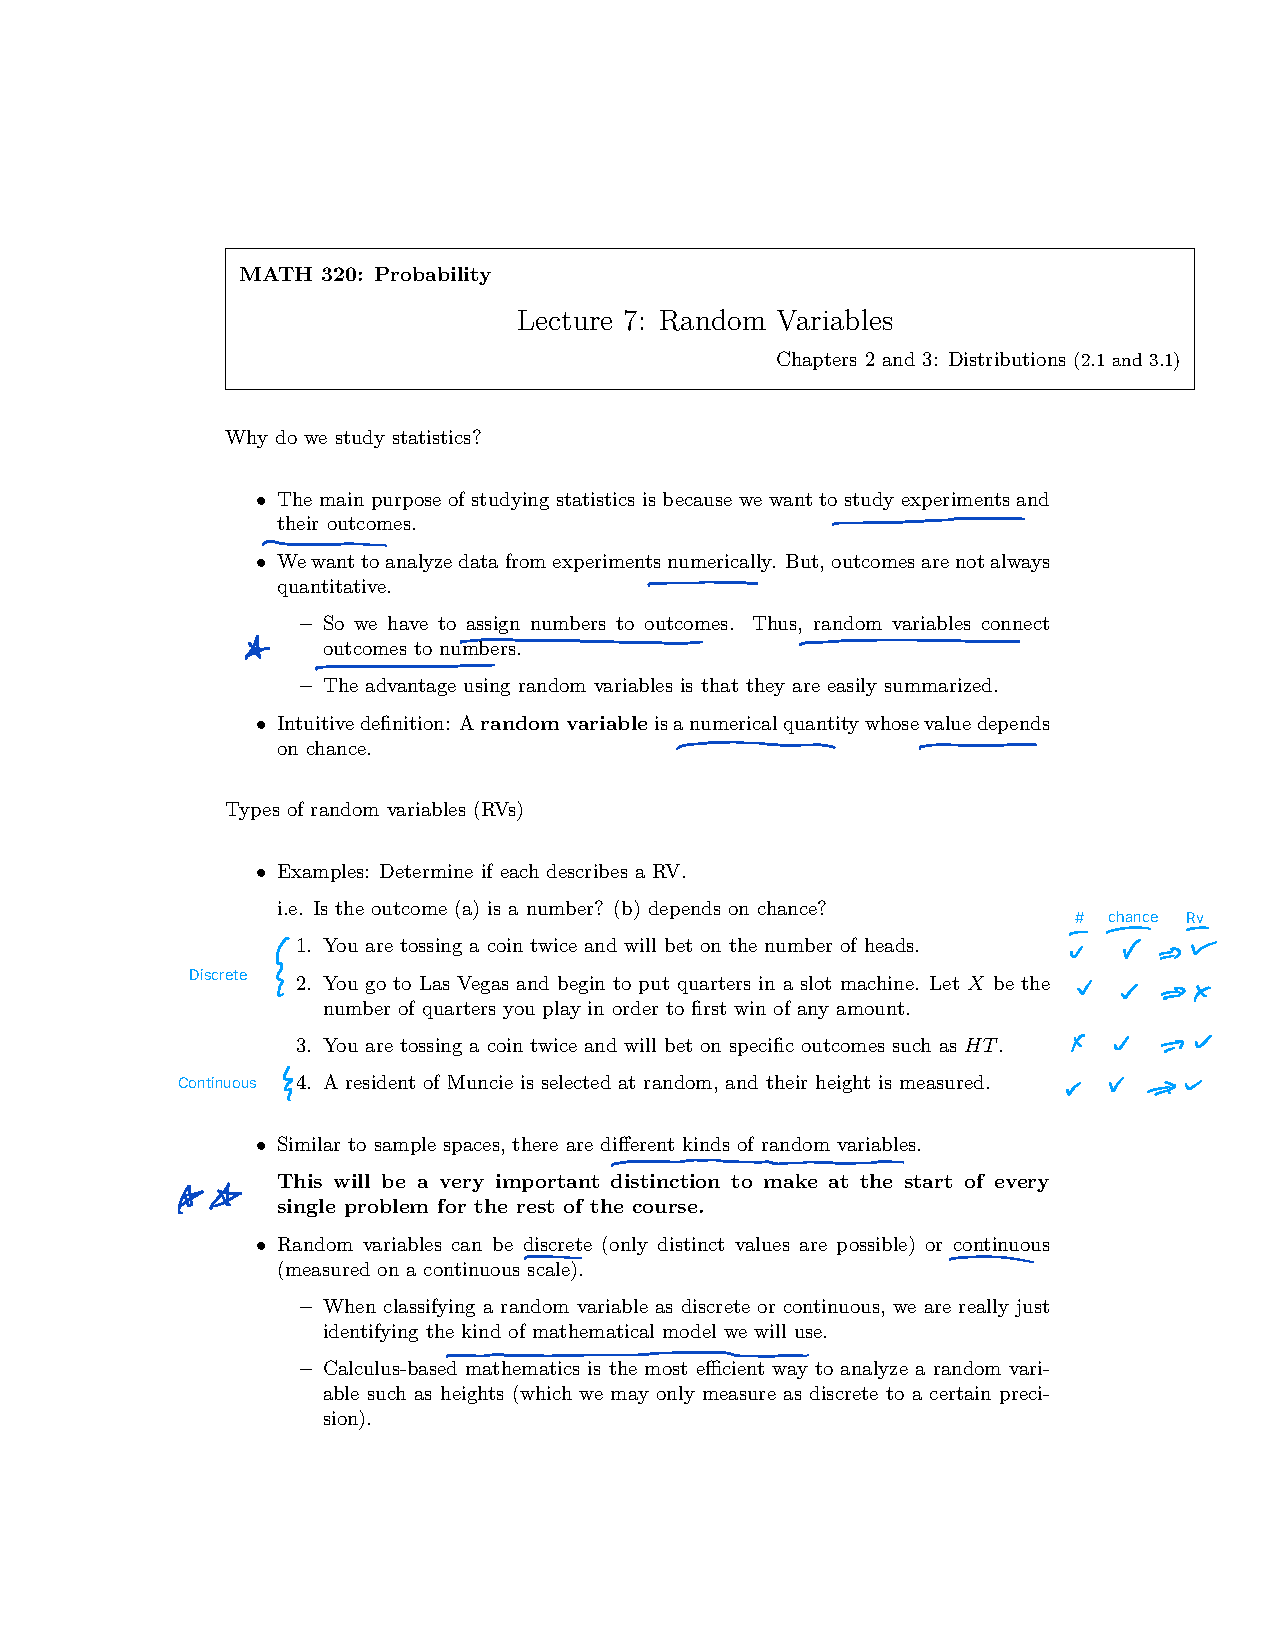
\includepdf[pages=-]{lecture-7-COMPLETED.pdf}\newpage
%----------------------------

%----------------------------
\subsection{Lecture 8 -- Distribution Functions}
\includepdf[pages=-]{lecture-8-COMPLETED.pdf}\newpage
%----------------------------

%----------------------------
\subsection{Lecture 9 -- Summary Measures}
\includepdf[pages=-]{lecture-9-COMPLETED.pdf}\newpage
%----------------------------

%-------------------------------------------------------------------------
\section{Test 3}
%-------------------------------------------------------------------------

\secttoc

%----------------------------
\subsection{Lectures 10 -- Discrete Distributions}
\includepdf[pages=-]{lecture-10-COMPLETED.pdf}\newpage
%----------------------------

%----------------------------
\subsection{Lectures 11 -- Continuous Distributions}
\includepdf[pages=-]{lecture-11-COMPLETED.pdf}\newpage
%----------------------------

%----------------------------
\subsection{Lectures 12 -- Moment Generating Functions}
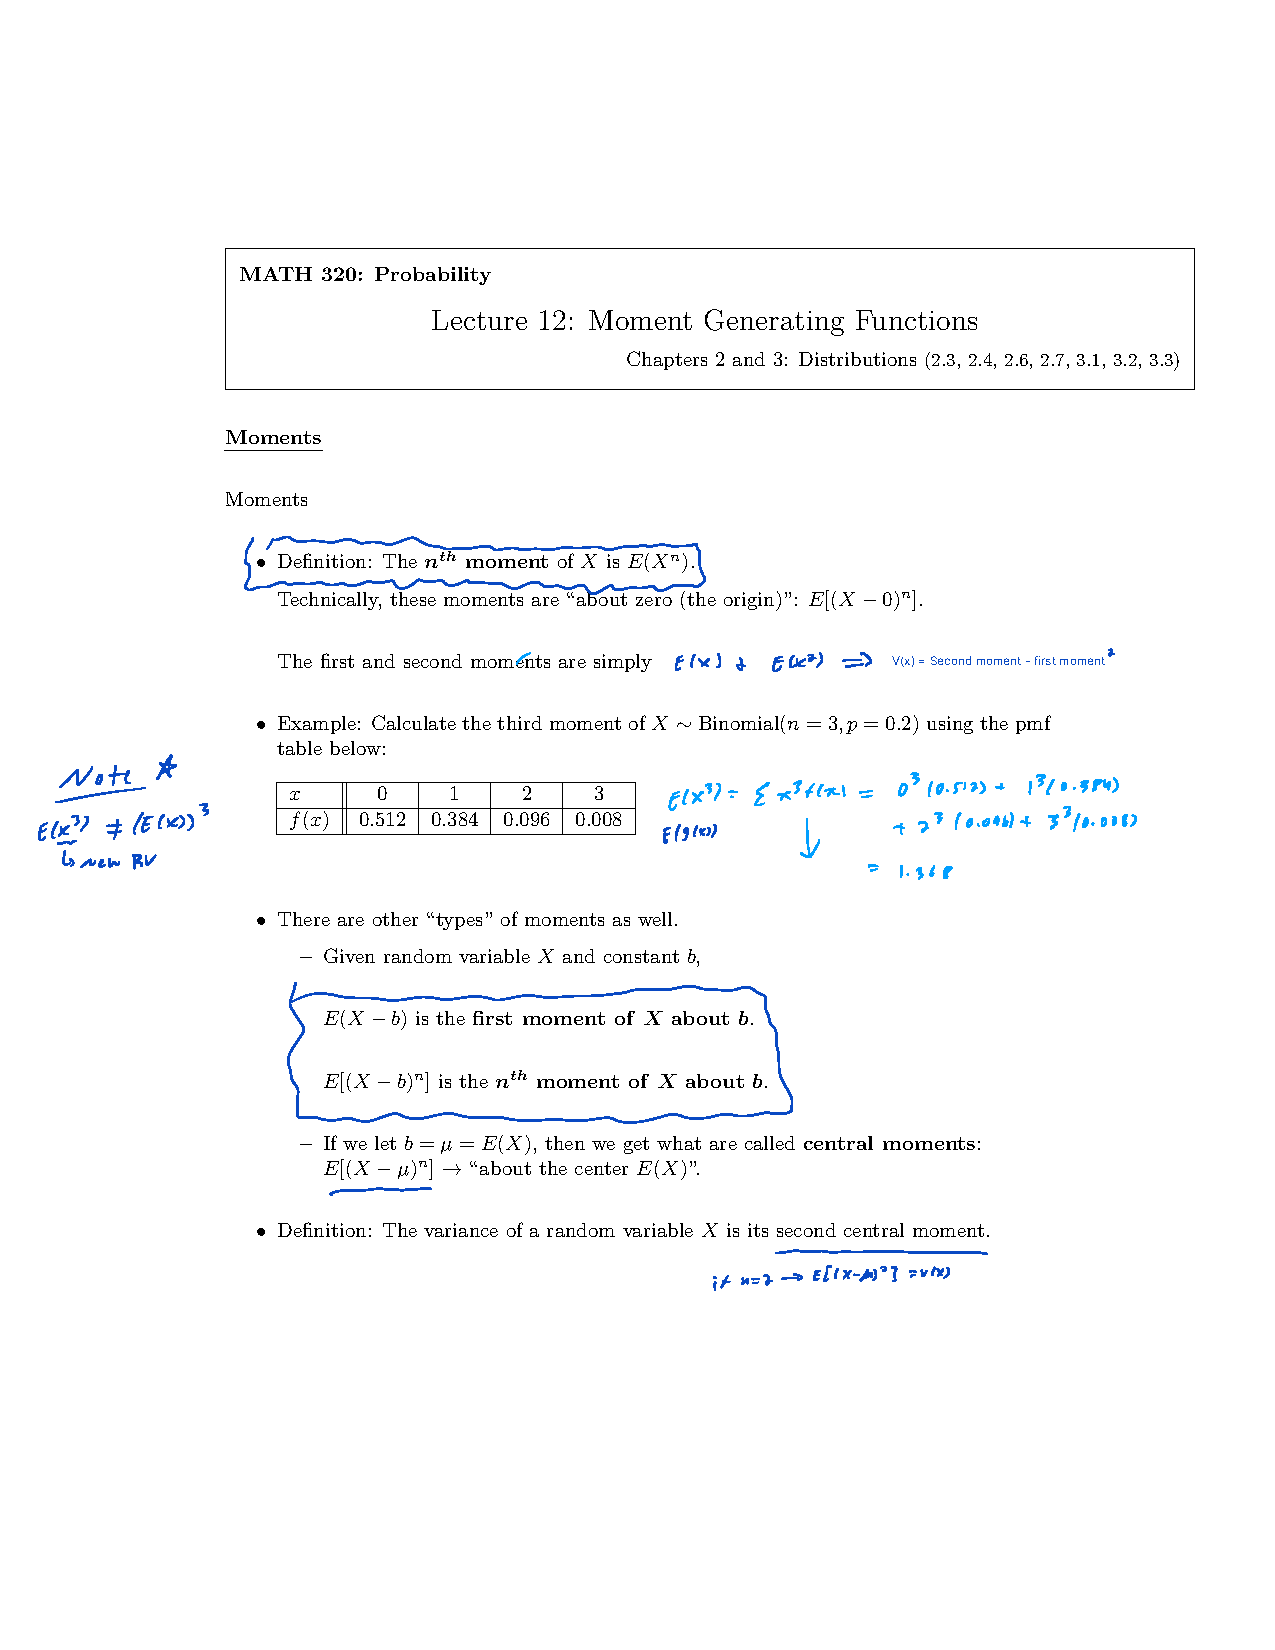
\includepdf[pages=-]{lecture-12-COMPLETED.pdf}\newpage
%----------------------------

%-------------------------------------------------------------------------
\section{After Test 3}
%-------------------------------------------------------------------------

\secttoc

%----------------------------
\subsection{Lectures 13 -- Functions of Random Variables}
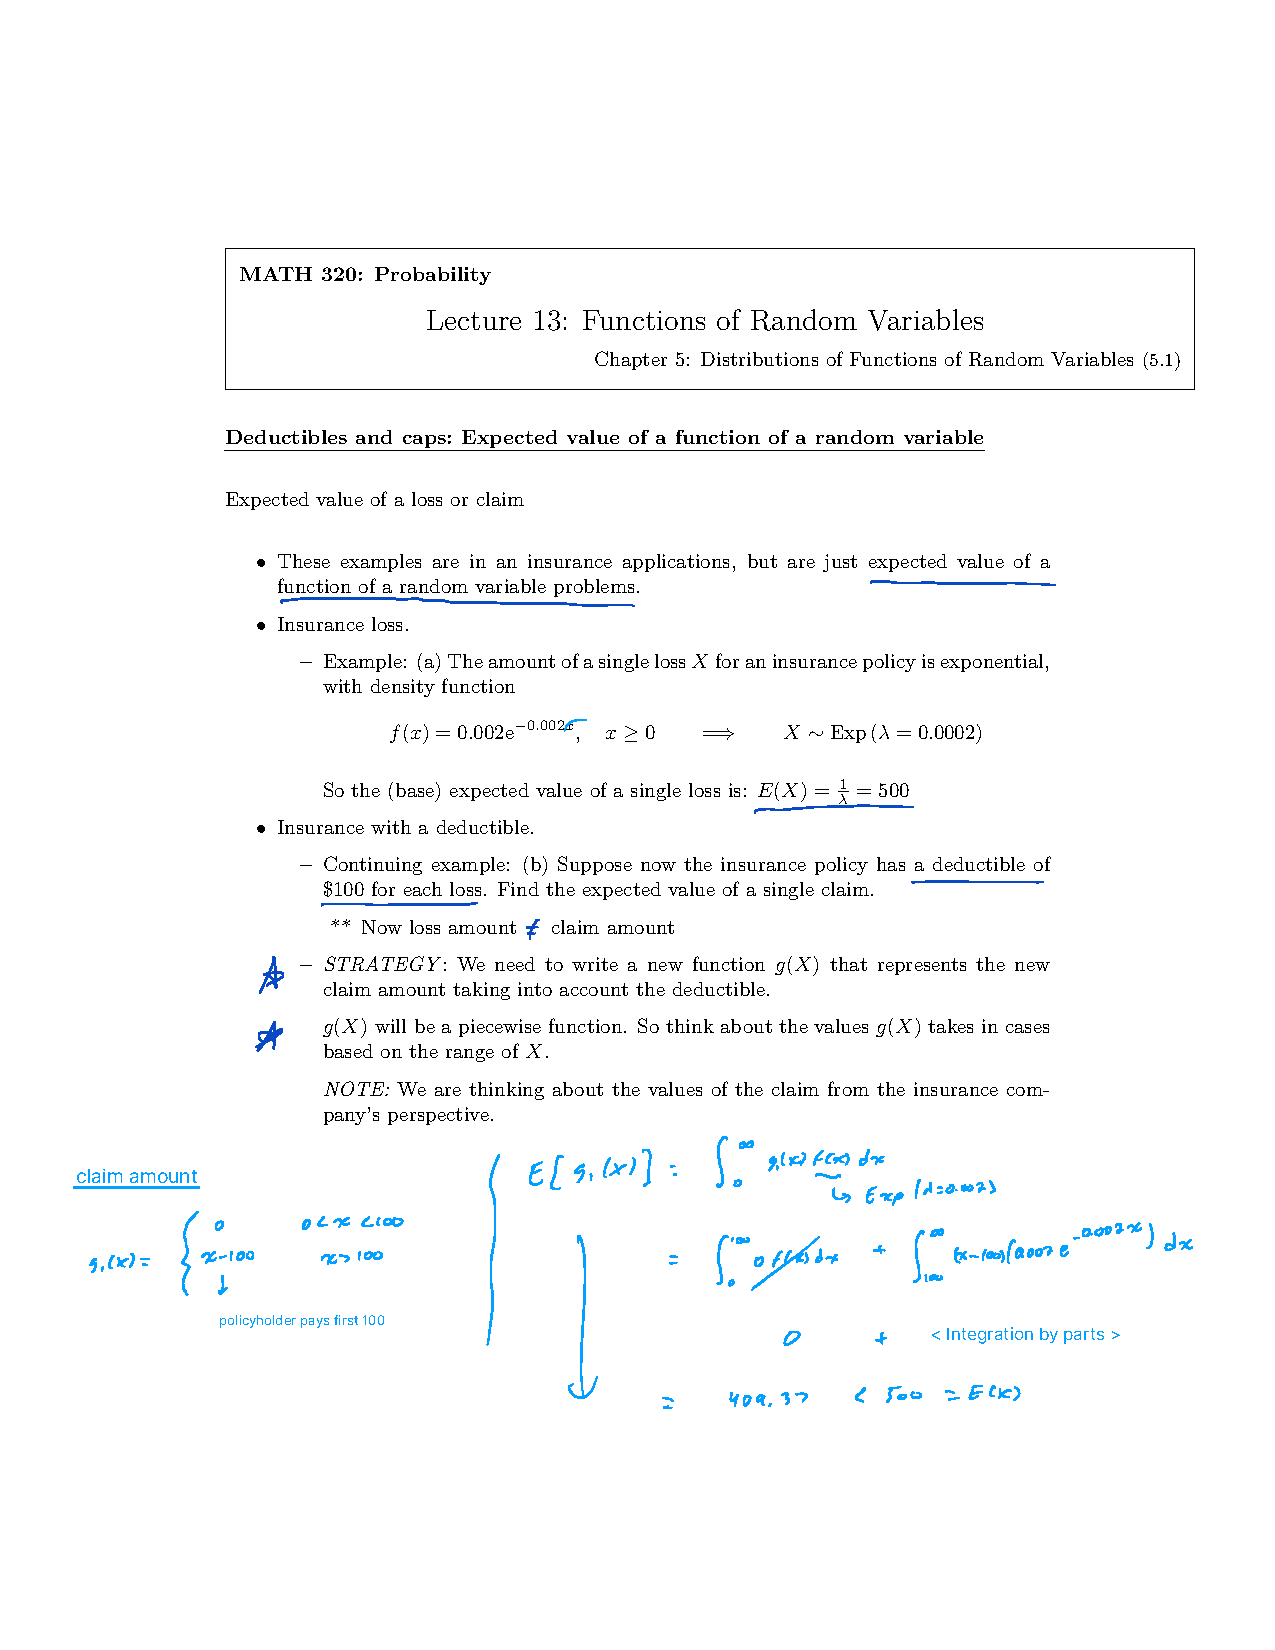
\includepdf[pages=-]{lecture-13-COMPLETED.pdf}\newpage
%----------------------------


\end{document}